\section{Learning}

\begin{frame}
	\frametitle{Organizational forgetting: Definitions}
	\begin{itemize}
		\item \textit{Organizational learning}: "change in the organization's knowledge that occurs as a function of experience" \citep[p. 31]{Argote2013}.
		\item \textit{Organizational forgetting}: "the loss, voluntary or otherwise, of organizational knowledge [which] often leads to a change in organizational capabilities because of the absence of some piece of knowledge" \citep[p. 1606]{DeHolan2004}.
		\note{Both forgetting and disruptions are thought to be sometimes positive, too, but I will not cover that here.\medbreak Disruption also sometimes desdribed as merely "interacting" with forgetting (Anderson \& Lewis 2014).\medbreak}
		\item \textit{Disruptions}: "organizational change-inducing events" \citep[p. 362]{Anderson2014}
		\note{Will have examples of disruptions in the next couple of slides.}
	\end{itemize}
\end{frame}

\begin{frame}
	\frametitle{\insertsection}
	\framesubtitle{Learning curve}
	\begin{figure}
		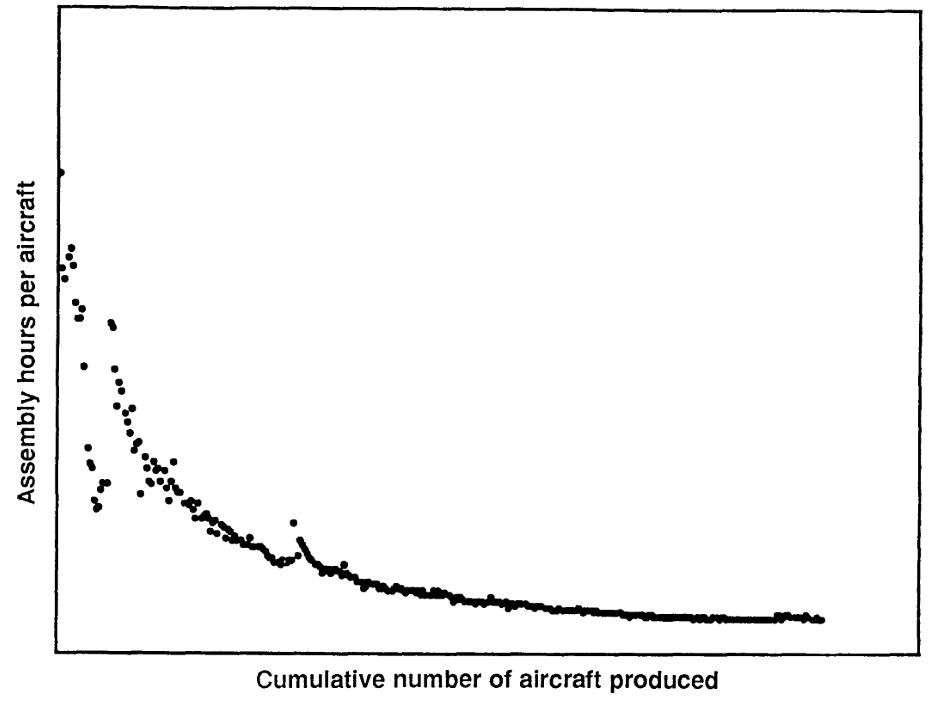
\includegraphics[height=5cm]{resources/learning_curve1.png}
		\caption{Relation between assembly hours per aircraft and cumulative number produced. Units omitted. From: \citet[p. 921]{Argote1990}}
		\note{You have probably seen this before.}
	\end{figure}
\end{frame}

\begin{frame}
	\frametitle{\insertsection}
	\framesubtitle{Disrupted learning}
	\begin{figure}
		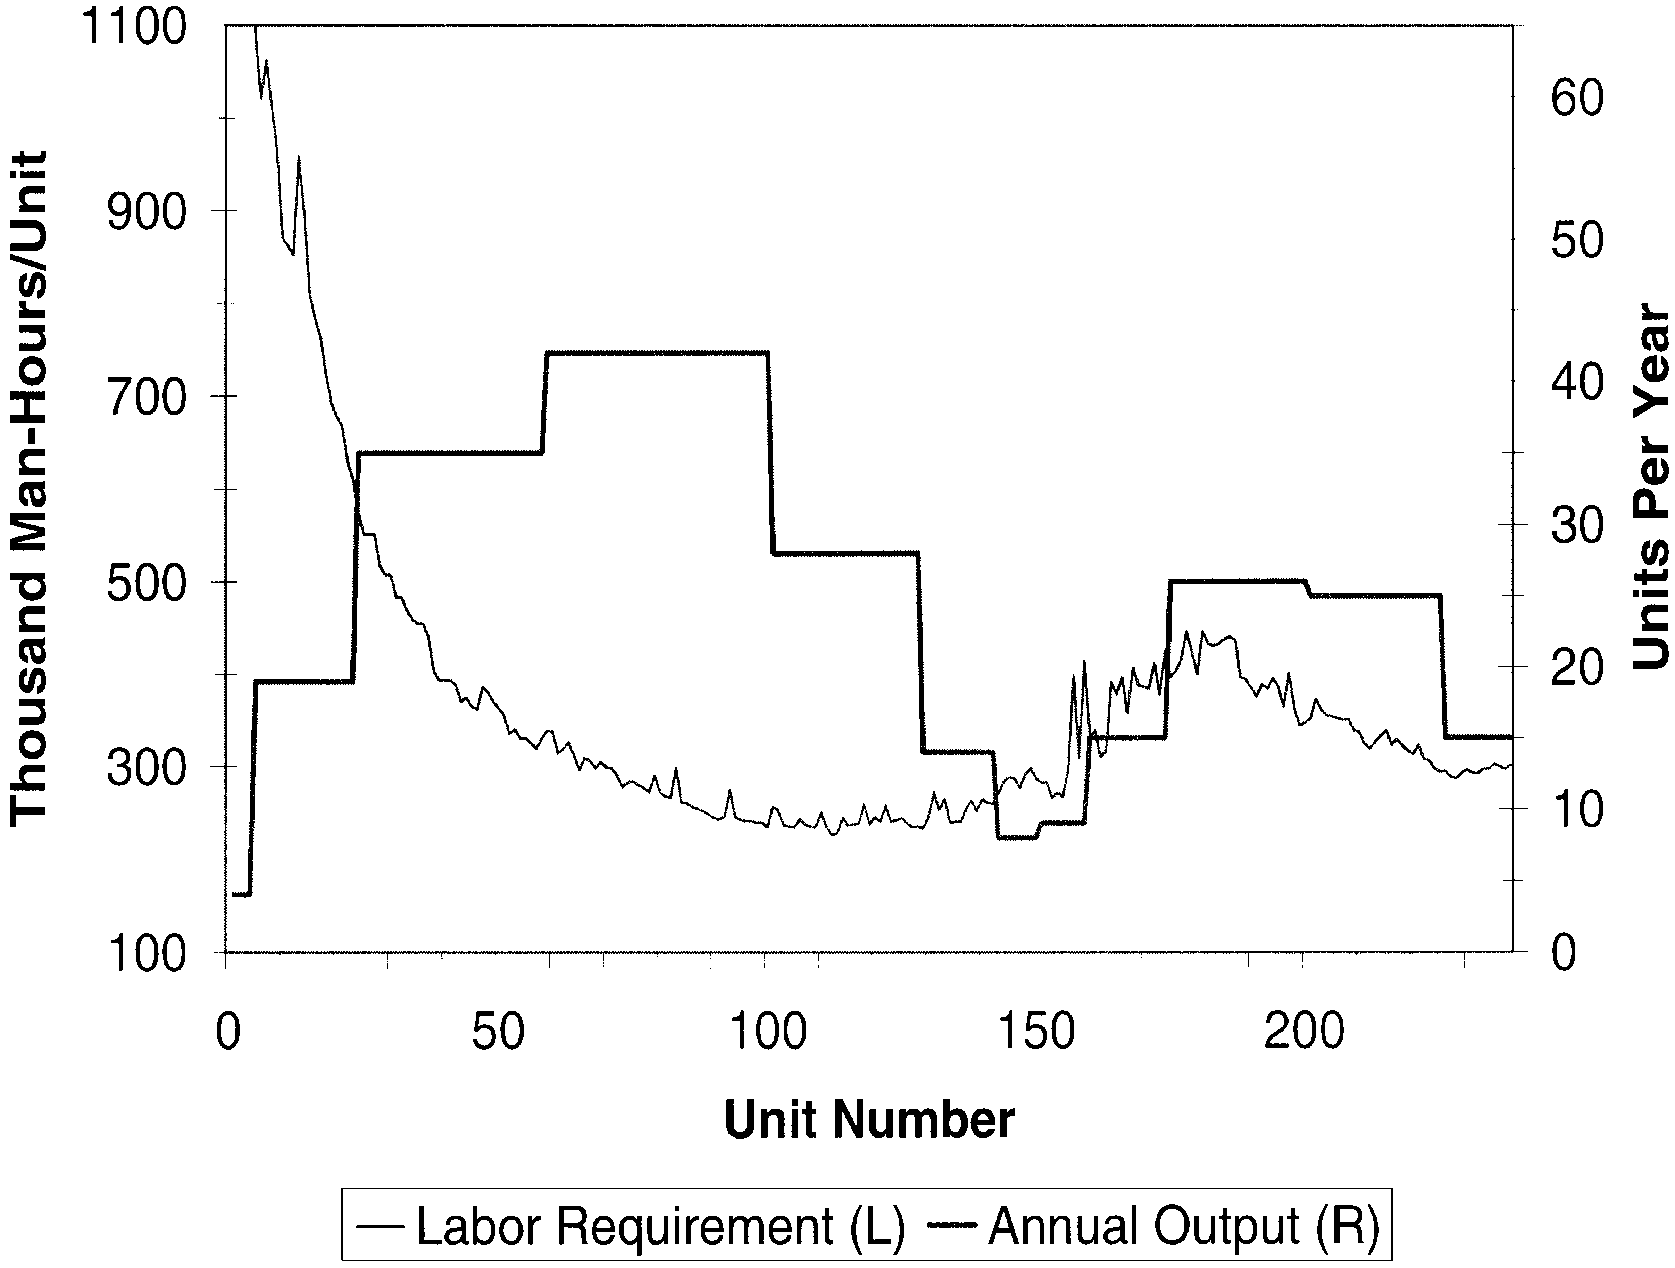
\includegraphics[height=5cm]{resources/learning_curve2.png}
		\caption{L-1011 Production: Direct Labor Requirement and Yearly Output. From: \citet[p. 1039]{Benkard2000}}
	\end{figure}
	\note{We see more than in the last picture. This is the production of the Lockheed L-1011. Famous for being an amazing plane, but a commercial failure. What happend here, around 150 units? Economic downturn, production was disrupted. Then, company decided the only way to break even is to produce a certain number of planes, but that did not happen.}
\end{frame}

\begin{frame}
	\frametitle{\insertsection}
	\framesubtitle{Disrupted learning}
	\begin{figure}
		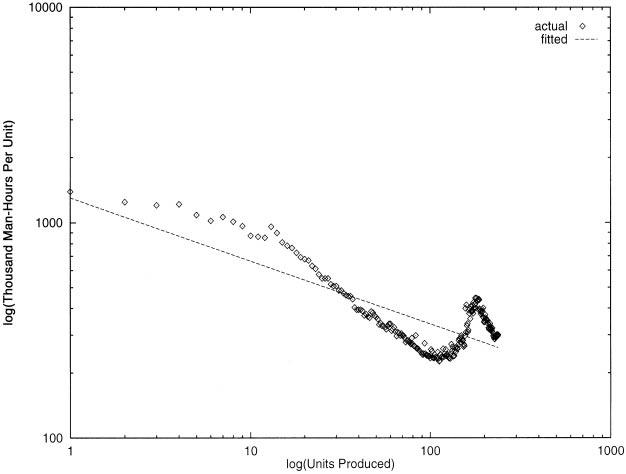
\includegraphics[height=5cm]{resources/learning_curve3.jpg}
		\caption{Traditional Learning Curve: All 238 (log-log). From: \citet[p. 1046]{Benkard2000}}
	\end{figure}
	\note{This is what actually happened. After Lockheed increased production again, the number of man-hours per plane actually increased for a while, before the price decreased again.}
\end{frame}

\begin{frame}
	\begin{block}{}
		\Huge Organizational forgetting
		\bigbreak		
		\normalsize Also known as knowledge depreciation
		\note{The Lockheed is a pretty famous example for this.}
	\end{block}{}
\end{frame}

\begin{frame}
	\frametitle{Organizational forgetting}
	\begin{itemize}
		\item Turnover \citep{DeHolan2004,Rao2006}
		\note{When a large number and/or key employees leave a company, and knowledge and/or networks are lost as a result.}
		\item Loss of recorded knowledge
		\item Technology becoming irrelevant
		\item Decay of social networks \citep{Argote2013_3,Argote1990,Thompson2007}
		\item Disruption
		\item 
		\begin{itemize}
			\item Internal
				\begin{itemize}
					\item Disruption of regular production 
					\item Technology \citep{Amburgey1993,Edmondson2001}
					\item Restructuring/reorganization/layoffs (or even hirings) \citep{Benkard2000,Anderson2014}
						\note {Which is also acknowledges in the wider learning literature.\medbreak}
				\end{itemize}
			\item External
				\begin{itemize}
					\item Economic cycles \citep{Rockart2019}
					\item Natural disasters \citep{Anderson2014}
				\end{itemize}
		\end{itemize}
	\end{itemize}
	\note{Organizational disruption is special case of organizational forgetting. Disruption can stem from inside, or outside of the organization.}
\end{frame}


